% \setcounter{figure}{0}
% \setcounter{listing}{0}

\pagenumbering{arabic}
\renewcommand*{\thepage}{B-\arabic{page}}



\chapter{Description of Digital Submission \label{cha:cdrom} }

\textbf{Thesis Evidence Number:} \\ \myEvidenceNumber

Obsah elektronického média je väčší ako \texttt{1GB} a preto je odovzdaný vedúcemu záverečnej práce (doc. Ing. Giang Nguyen Thu, PhD.).


\textbf{Name of submitted archive:} \texttt{DP\_MenoPriezvisko.zip}
    % \texttt{BP\_MenoPriezvisko.zip}


The digital part included in the thesis contains the following files:
\begin{itemize}
    \item Ubuntu OS: run in command line \texttt{\$ tree} to get a directory structure as below.
    \item Inspiration from \textit{https://github.com/FIIT-ISA/cookiecutter-data-science}
\end{itemize}


\begin{verbatim}
    ROOT // Root directory.
    │
    ├── flatbuffers // This flatbuffers director
    └── scheme
\end{verbatim}

\begin{figure}[h]
    \begin{centering}
    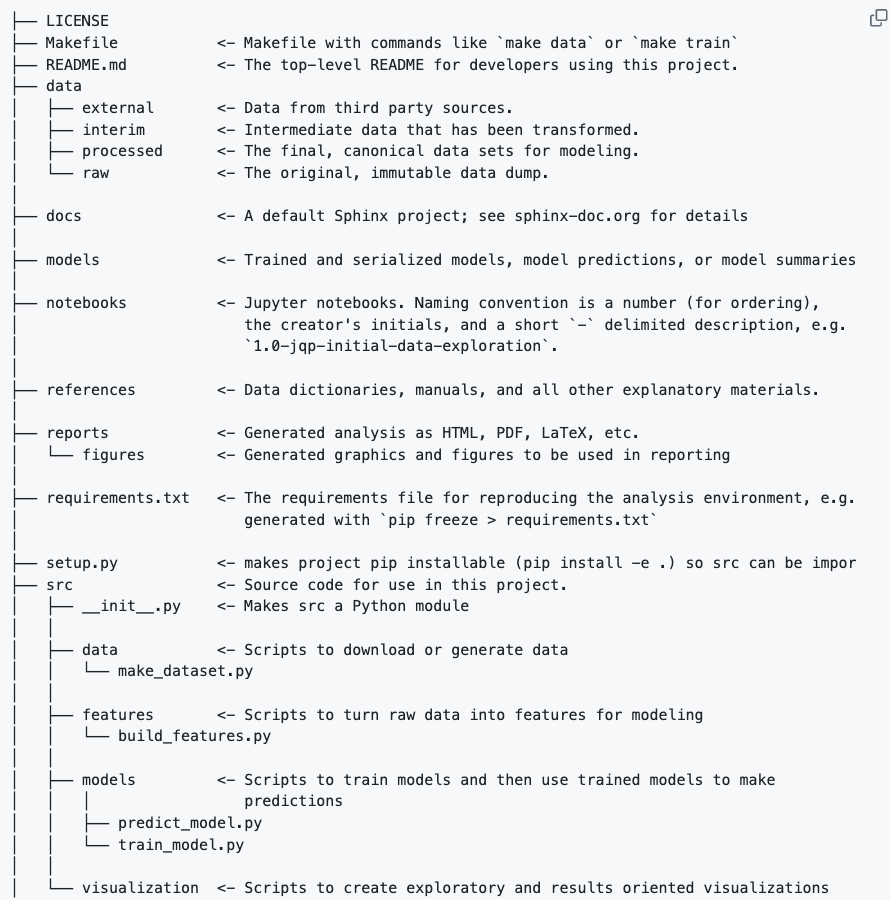
\includegraphics[width=\textwidth]{appendices/zip-file-structure.png}
    \par\end{centering}
\caption{The structure of the ZIP file \label{fig:zip-file-structure}}
\end{figure}



\chapter{Technical Documentation}
\label{chapter:Technical-Documentation}

\section{Installation Manual}
\label{sec:Installation-Manual}

\begin{enumerate}
    \item Clone the project from the Git repository (URL) OR unzip the ZIP file ...
    \item Run \emph{pip install -r requirements.txt} in the root folder of the project
    \item Run \emph{python -m spacy download en} to have the data corpus ...
\end{enumerate}


\section{User Manual / Používateľská príručka}
\label{sec:User-Manual}

\begin{enumerate}
    \item Spustenie programu funguje pomocou hlavného Python súboru \emph{main.py} príkazom \emph{python main.py}. 
    
    \item Po spustení programu sa zobrazí grafické rozhranie programu v ktorom sa dá hneď na hlavnej obrazovke spustiť sumarizácia pre jeden vstupný súbor.

    \item Tlačidlami v hornej časti obrazovky sa dá presúvať medzi funkcionalitami programu ako je viac súborová sumarizácia alebo zobrazovanie článkov. Na týchto obrazovkách sa tlačidlom \emph{Back to main menu} dá vrátiť späť na hlavnú obrazovku.

\end{enumerate}

Screenshot(s) používateľského grafického rozhrania (GUI) ako obrázok (Figure)

(Another variant without GUI: ) The main objective of this work is to ... Several case studies were presented that examine the capabilities of ... to show the feasibility and achievability of ... 
Users in our work are considered to work directly with the code as described in Section~\ref{sec:Installation-Manual}.



\section{Developer Manual}
\label{sec:Developer-Manual}

if needed then add ...